\chapter{STATE OF THE ART}
\normalsize{In this chapter, the design, the use and the architecture of the reflector tile will be explained. Moreover, the already existing analyses and results will be discussed to give context and insight about the situation and the functionning of this system.}
\section{THE \acrshort{ECRH} \acrshort{TZM} REFLECTOR TILE ASSEMBLY}
\normalsize{The reflector tile is used to reflect the \acrshort{ECRH} beam back into the plasma to limit energy loss. This reflector tile is placed in a particular position inside of the stellarator.}
\begin{figure}[h!]
    \centering
    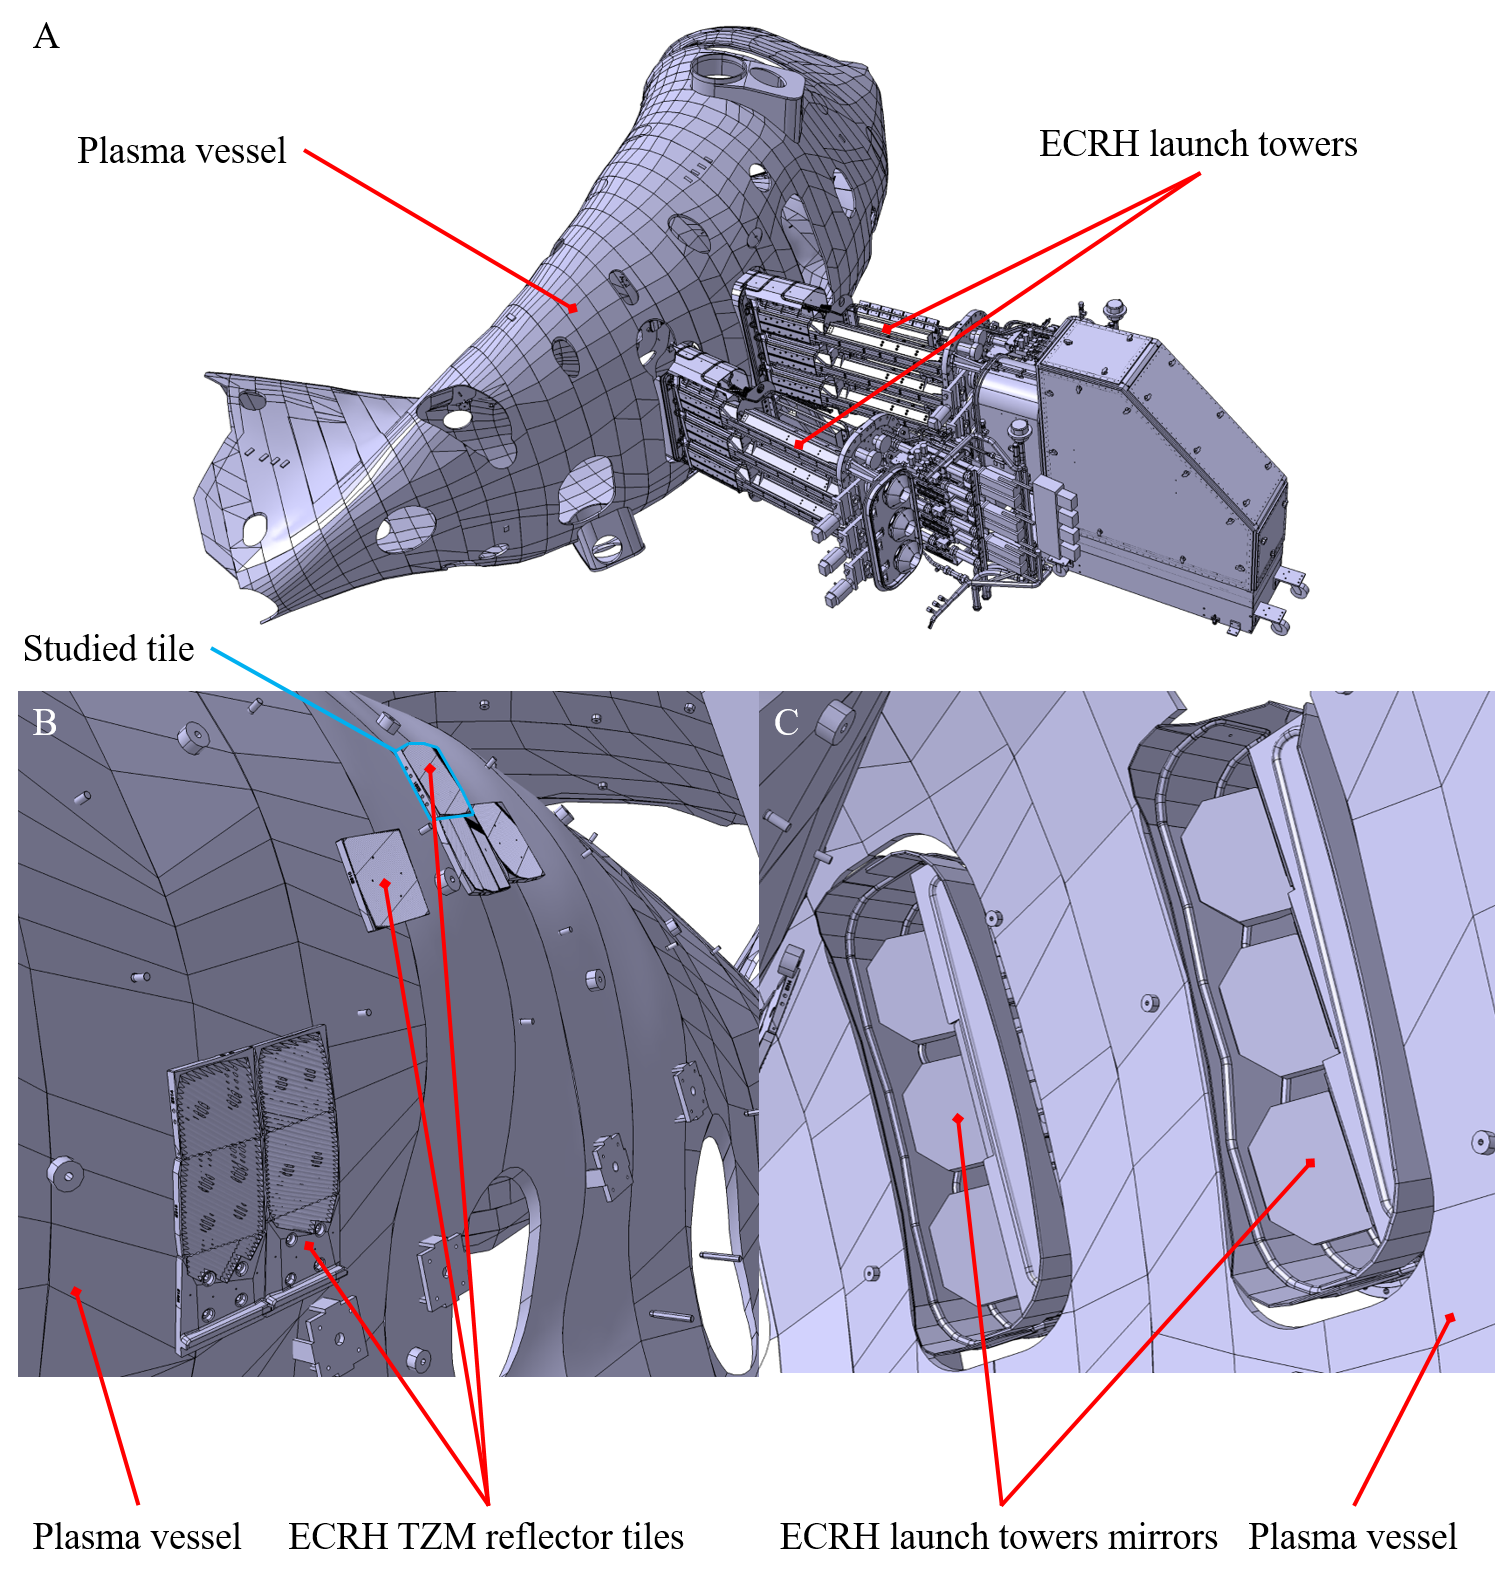
\includegraphics[width=1\textwidth]{figures/ecrhposition2.png}
    \caption{\it Different views of the \acrshort{ECRH} launchers and reflector tiling}
    \label{fig:fig_3_1}
\end{figure}
\\
\normalsize{The different views from figure \ref{fig:fig_3_1} are:
\begin{itemize}
    \item A: View of the plasma vessel and the two \acrshort{ECRH} launchers
    \item B: View of the \acrshort{ECRH} \acrshort{TZM} reflector tiles
    \item C: View of the launcher mirrors
\end{itemize}
}
\normalsize{\indent The reflector tiles face the plasma and are a component of the \acrshort{PFCs} and are placed in front of the \acrshort{ECRH} launch towers. A reflective alloy made of titanium zirconium and molybdenum abbreviated \acrshort{TZM} was chosen to build the reflector tile. The reflector tile is mounted on a copper chromium zirconium heat sink that is brazed onto a stainless steel cooling pipe. The \acrshort{ECRH} reflector tile is placed on one of the modules composing the in-vessel components or \acrshort{KiP}.}
\\
\break
\normalsize{\indent The reflector tile has a simple assembly. The \acrshort{TZM} reflector tile is held in place using holding pins screwed on the side of the tile. The holding pins hold the head of the bolt back. A nut is screwed on the bolt and using a $270 \si{\degree}$ turn, the nut pushes again a stack of three INCONEL Belleville washers. The washers, acting like a preloaded spring, push agains't the \acrshort{CuCrZr} heat sink, applying a force on the \acrshort{Sigraflex} thermal gasket which thermally separates the \acrshort{TZM} tile and the \acrshort{CuCrZr} heat sink.}
\begin{figure}[h!]
    \centering
    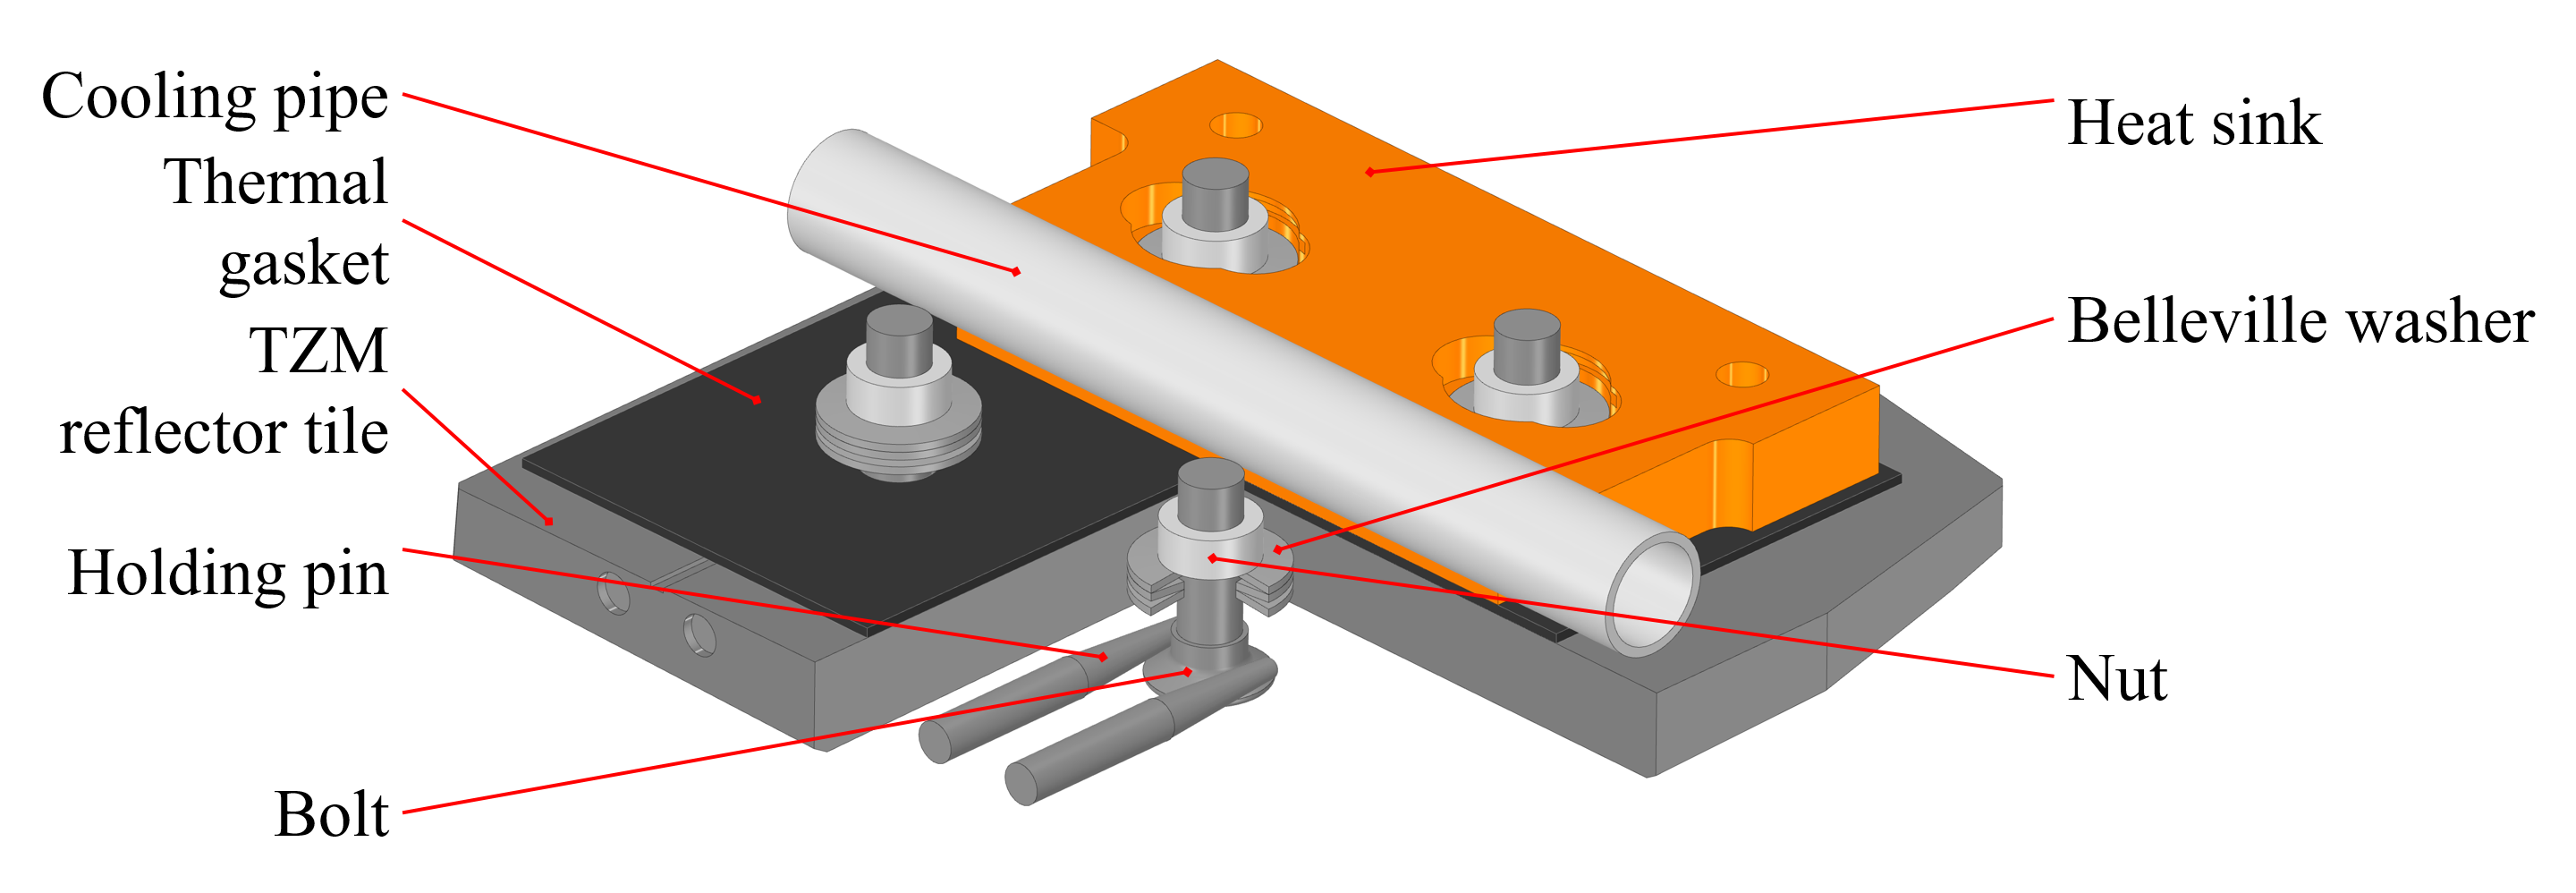
\includegraphics[width=1\textwidth]{figures/montage2.png}
    \caption{\it Components and montage of the reflector tile assembly}
    \label{fig:fig_3_2}
\end{figure}
\\
\break
\normalsize{\indent The reflector tile will be exposed to high heat fluxes that can be decomposed into two different sources (those two different heat sources will be implemented in the \acrshort{FE} model for the analysis):
\begin{itemize}
    \item Plasma heat load {\it (radiative and convective heat loads)}
    \item \acrshort{ECRH} heat load
\end{itemize}
In a real powerplant condition (using Deuterium-Tritium mix as fuel), the \acrshort{PFCs} would be exposed to other physical constraints and scenarios, in particular the neutron flux generated by the fusion reaction (generating defects and transmutations in the materials) or the diffusion of hydrogen into the material of the first walls potentially negatively affecting the mechanical properties and behavior of the first wall component materials. Highly dynamic phenomena such as Edge Localized Modes (\acrshort{ELMs}) or disruptions can also be challenging for the first walls.}
\\
\break
\normalsize{\indent In the case of \acrshort{W7-X}, in particular for \acrshort{OP2}, no neutrons will be produced nor the heat fluxes reach powerplant-like values. It is still important to keep these considerations in mind to design the most effective \acrshort{PFCs} and prepare for burning plasma, especially for reflector tiling or \acrshort{NBI} dump tiling. }
\\
\break
\normalsize{\indent Those constraints can be summarized:}
\begin{figure}[h!]
    \centering
    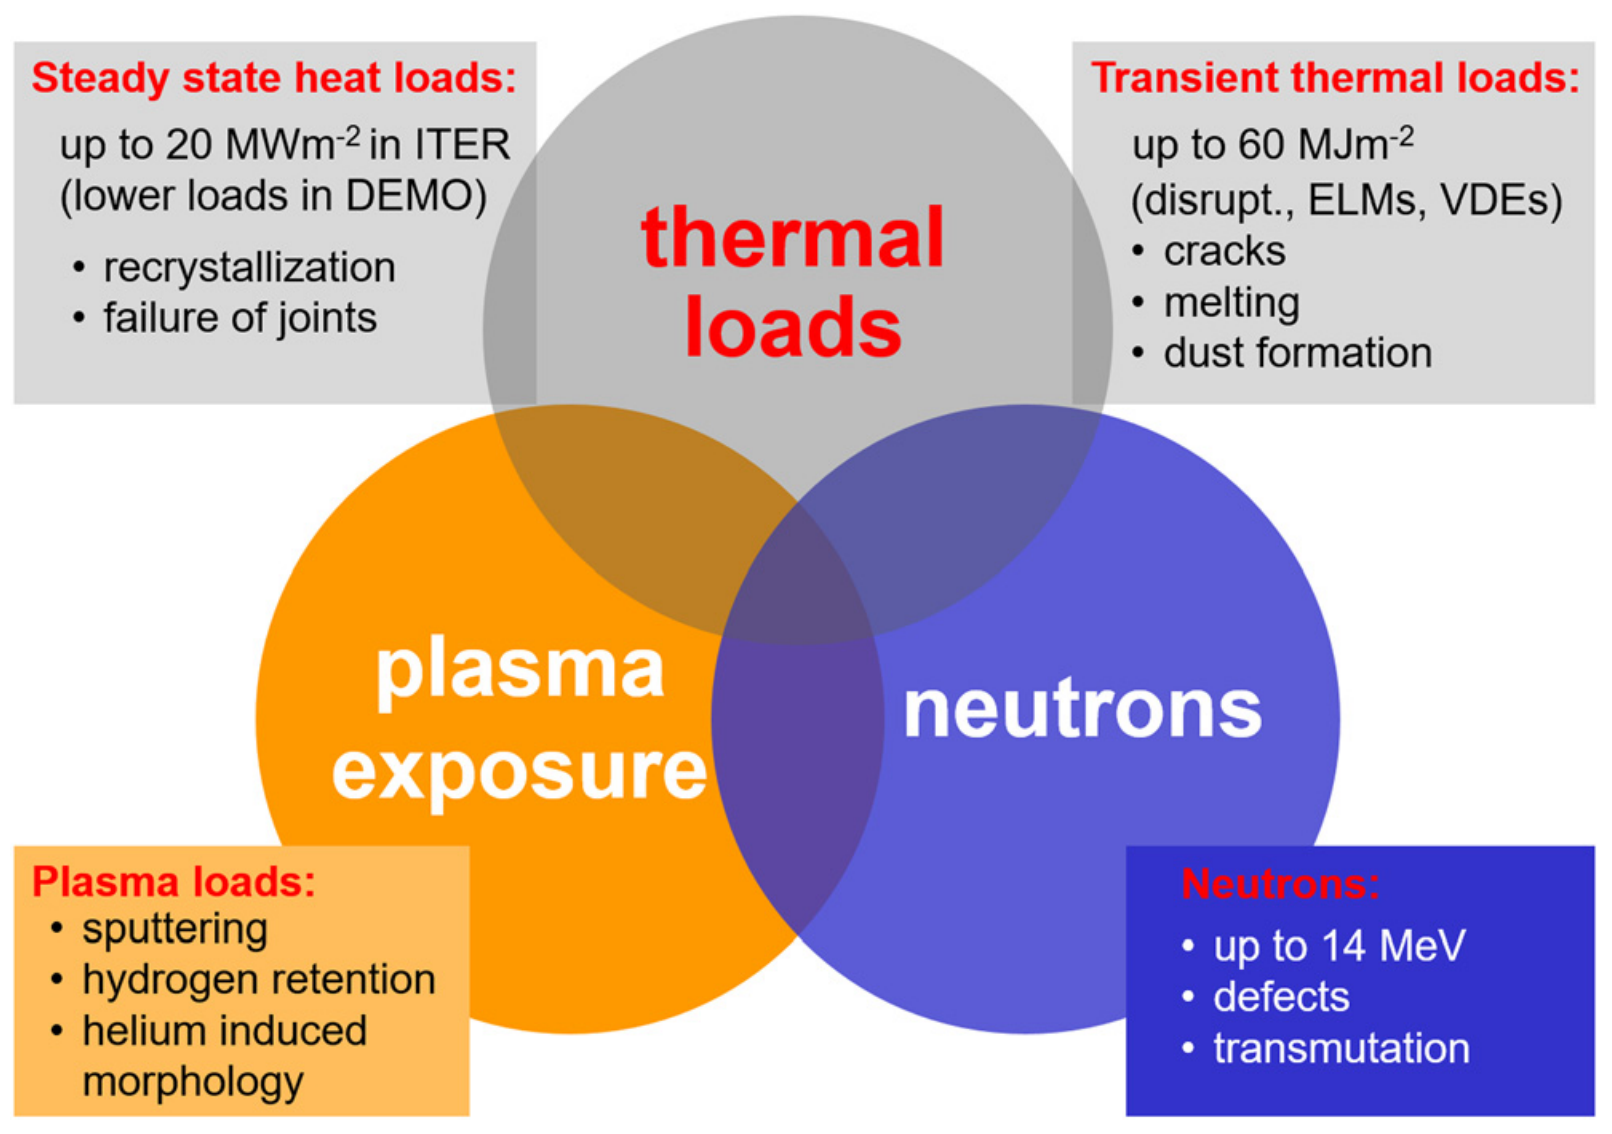
\includegraphics[width=.7\textwidth]{figures/physicalconstraintsBurningPLasma.png}
    \caption{\it Physical constraints for burning plasma \acrshort{PFCs} \cites{Linke_2019}}
    \label{fig:fig_3_3}
\end{figure}
\\
\section{PREVIOUS ANALYSES OF THE ECRH REFLECTOR TILE}
\normalsize{In order to reflect the \acrshort{ECRH} beam into plasma back, some \acrshort{TZM} tiles were suggested to substitute the \acrshort{BM} graphite tiles in specific positions. The idea was to limit power loss due to absorption of the \acrshort{ECRH} beam by the graphite tiles. After \acrshort{OP1}.2 it was decided to increase the size of the \acrshort{TZM} tile. Due to the fact the tile has been never analyzed in details, corresponding thermal and structural analysis is to be performed to assess the performance of the tile in \acrshort{OP2}.}
\\
\break
\normalsize{\indent For \acrshort{OP2}, plasma discharge duration will be increased thus exposing the \acrshort{PFCs} to longer heat loads. The “worst” tile had been selected during discussion between Victor Bykov and Torsten Stange and was analyzed. Those analyses aimed to give insight about the thermal and structural integrity of the \acrshort{ECRH} reflector tile during the plasma discharges with \acrshort{OP2} specifications.}
\\
\begin{figure}[h!]
    \centering
    \includegraphics[width=.85\textwidth]{figures/JFellingerFEModel2.png}
    \caption{\it FE model of the tile assembly \cite{Fellinger_2013}}
    \label{fig:fig_3_4}
\end{figure}
\\
\break
\normalsize{\indent Different analyses such as transient thermal and fatigue analyses were performed by various engineers to assure proper functioning of the tile. One of those analyses were performed by Joris Fellinger in 2013 and was the thermal-mechanical assessment of heat shields and baffles \cites{Fellinger_2013}. The analyses were performed on a simplified model $see \ figure \ \ref{fig:fig_3_4}$ of the tile and calculated using Dassault Systèmes Abaqus. Perfect thermal contact between the parts was also assumed to simplify the model. The heat pulse was simplified to be a step signal lasting for about $90 \ s$. Models for fatigue dimensionning and material properties were defined and used in this work. Thermal properties of the differents materials used are also given and important for the rest of the work.}
\\
\break
\normalsize{\indent The effect of the boundary conditions, in particular restraining the axial displacement of the the steel cooling pipe has a non-negligible and detrimental influence on the plastic strain \cites{Fellinger_2013}. This conclusion is going to be seen later in this work regarding the structural analysis.}
\\
\break
\normalsize{\indent In this work, a discussion about the thermal performances of the brazing between the heat sink and the cooling pipe or the Sigraflex thermal gasket also stated that these moderatly affected the heat transfer within the tile assembly. On the other hand, the annealing of alloys and the temperature-dependant mechanical properties are a concern and the issue of having uncertain annealing of the \acrshort{CuCrZr} due to termal activation arose \cites{Fellinger_2013}. This will be an issue discussed later in the topic of this work.}
\\
\break
\normalsize{\indent Later, Jiawu Zhu was tasked to analyse the behavior of the tile and performed a complete thermo-mechanical analysis of the tile assembly. The model used by J. Zhu was quite different from the model of J. Fellinger because it featured the actual geometry of the reflector tile. The whole reflector tile as well as the thermal gasket, heat sink and cooling pipe were implemented in the model. the bolting system also included a simplified version of the Belleville washers and the bolts didn't have the same geometry.}
\begin{figure}[h!]
    \centering
    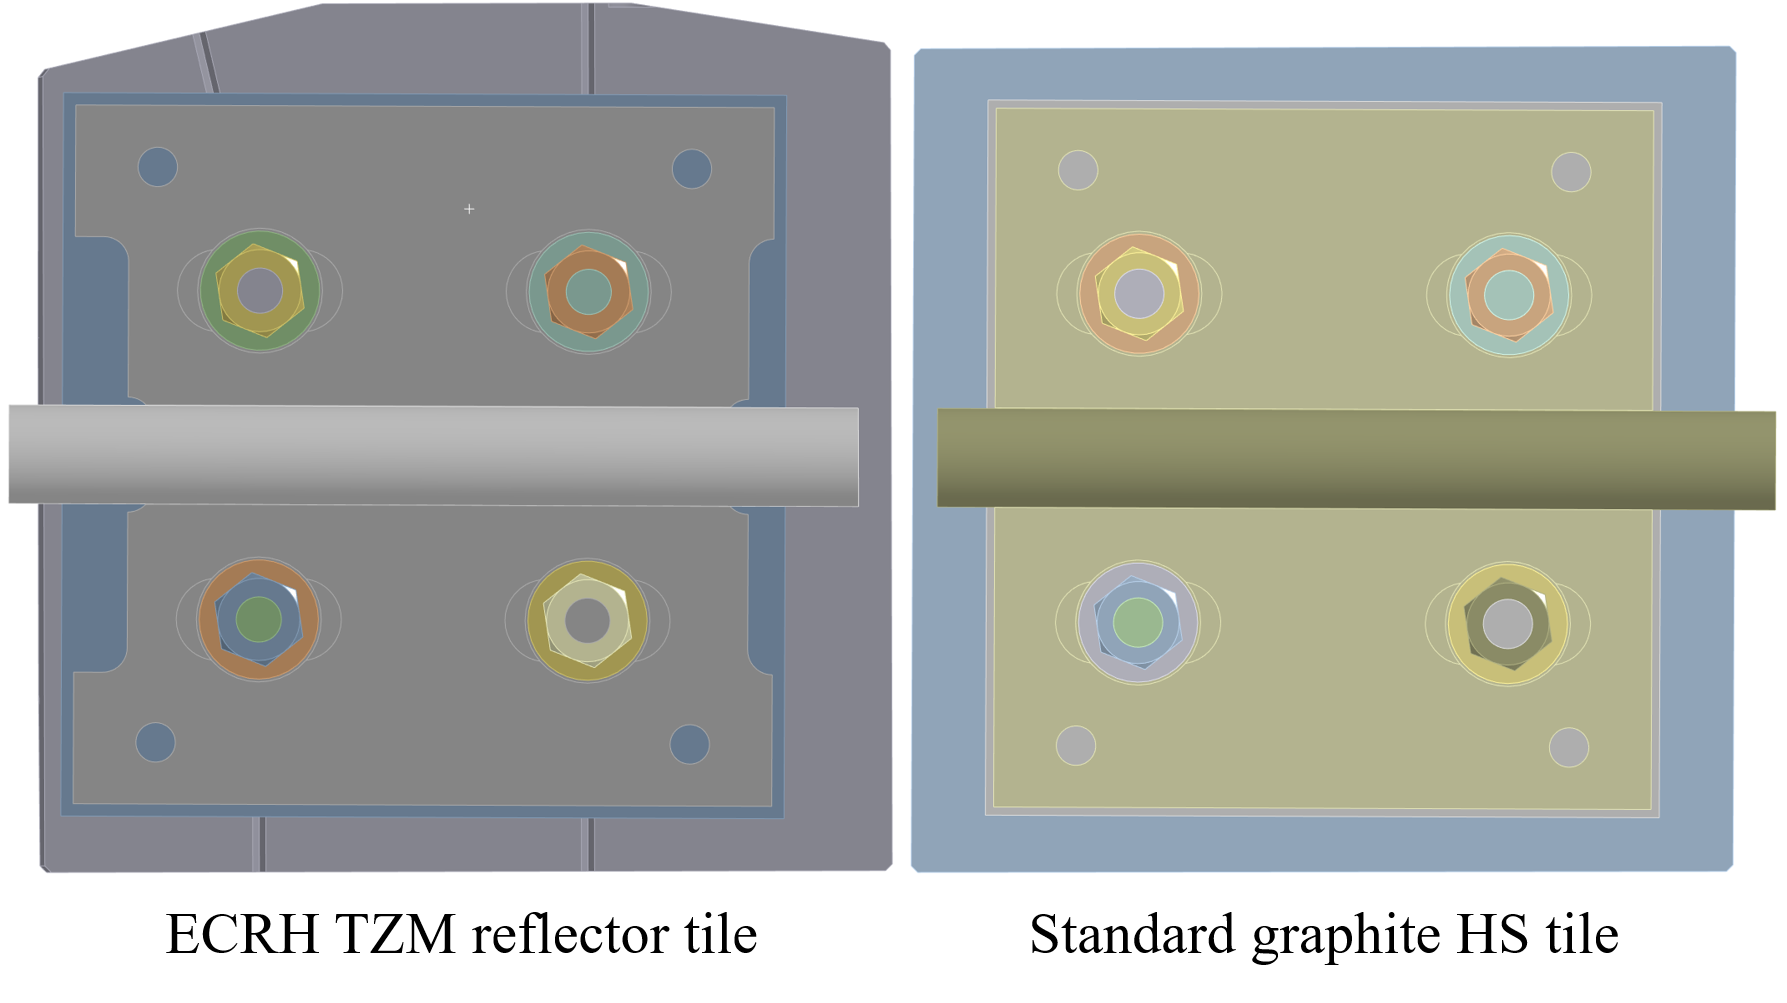
\includegraphics[width=.81\textwidth]{figures/jZhumodel.png}
    \caption{\it Model of the tile assembly \cite{zhu_parametric_2019}}
    \label{fig:fig_3_5}
\end{figure}
\\
\normalsize{\indent The analyses carried out by J. Zhu included another graphite tile of the heat shield to compare the results. The results were divided into two categories:
\begin{itemize}
    \item Thermal analysis
    \item Structural analysis (ie. fatigue analysis)
\end{itemize}
For the thermal analysis, the plasma heat load was initially $250 \unit{kWm^{-2}}$ and the \acrshort{ECRH} heat flow was $912 \unit{W}$ over a gaussian distribution to model the beam stray radiation. The results showed overheating of the \acrshort{CuCrZr} heat sink (in steady-state operation) and the plasma heat load was subsequently lowered to avoid reaching critical temperature of the bronze alloy of the heat sink. The heat flux was lowered to $220 \unit{kWm^{-2}}$ which represents {\bfseries $88 \unit{\%}$ of the specified heat load for \acrshort{OP2} (which is not enough to respect the operational specifications of \acrshort{OP2})}. The thermal analysis was redone $(see \ \ref{fig:fig_3_6})$ with the new heat load and showed acceptable temperature field for the heat sink. The issue with the recrystallization (as \ stated \ in \ \cite{Fellinger_2013}) of the \acrshort{CuCrZr} still is relevant for these analysis.}
\begin{figure}[h!]
    \centering
    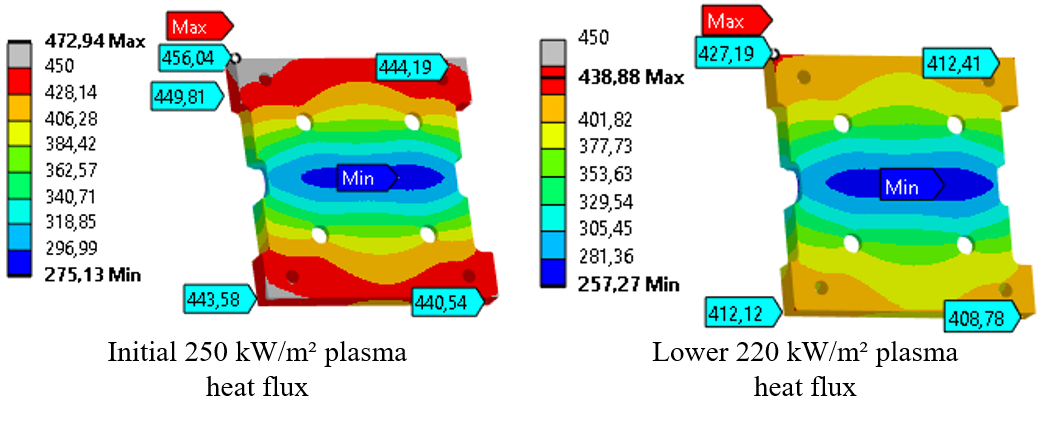
\includegraphics[width=1\textwidth]{figures/jZhuHS250vs220II.png}
    \caption{\it Temperature field (in [\si{\degree}C]) of the \acrshort{CuCrZr} heat sink for the two heat fluxes \cite{zhu_parametric_2019}}
    \label{fig:fig_3_6}
\end{figure}
\\
\break
\normalsize{\indent The structural analysis of the tile assembly was done by importing the temperature field in the mechanical analysis. one end of the cooling pipe is fixed and the other one let loose. The bending of the whole assembly is thus not constrained. The main point of concern was the assumption of perfect brazing between \acrshort{CuCrZr} heat sink and the \acrshort{SS} cooling pipe. In reality, it is possible that cracks may exist in the braze connection which could end up initiating a crack damaging the brazed connection \cite{zhu_parametric_2019}. While fracture mechanics are known, establishing a framework to effectively model multi-material interface fracture expansion remains a challenge that is out of the frame for this task.}
\section{ISSUES OF THE MODEL}
\normalsize{After the analyses done by J. Fellinger and J. Zhu, different issues were shown. The first issue is one of the parameter for the cooling pipe. The value of the film coefficient for the cooling pipe convection used by J. Zhu in his study \cite{zhu_parametric_2019} was set to be $30 \unit{kWm^{-2}\si{\degree}C^{-1}}$. This value is unlikely to be realistic and was discussed to reach at most $18 \unit{kWm^{-2}\si{\degree}C^{-1}}$ with a mininum value of $15 \unit{kWm^{-2}\si{\degree}C^{-1}}$. This gives the range of $3 \unit{kWm^{-2}\si{\degree}C^{-1}}$. The reduction of the film coefficient could prevent optimal cooling and heat evacuation and needs to be assessed.}
\\
\break
\normalsize{\indent The recrystallization of the \acrshort{CuCrZr} alloy could also negatively impact the mechanical properties. This phenomena is still not well known in this case because of lack of material data. The structural and fatigue behavior are also to be redone for $250 \unit{kWm^{-2}}$. The material properties also need to be revised to taken into account new material properties.}
\\
\break
\normalsize{\indent With that in mind, it is possible to build a new numerical model based on revised boundary conditions and material properties.}